\section*{Pregunta 1}
\noindent Decimos que un árbol binario de búsqueda $T_1$ puede ser \textsc{right-converted} a un árbol binario de búsqueda $T_2$ si es posible obtener $T_2$ de $T_1$ por a tráves de una serie de llamadas a la operación \textsc{right-rotate}.
\begin{itemize}
    \item Da un ejemplo de dos árboles $T_1$ y $T_2$ tal que  $T_1$ no pueda ser \textsc{right-converted} en $T_2$.
    \item Demuestra que si un árbol $T_1$ puede ser \textsc{right-converted} a $T_2$, entonces $T_1$ puede ser \textsc{right-converted} usando $O(n^2)$ operaciones \textsc{right-rotate}.
\end{itemize} 


\subsection*{Respuesta}


\begin{itemize}
    \item Da un ejemplo de dos árboles $T_1$ y $T_2$ tal que  $T_1$ no pueda ser \textsc{right-converted} en $T_2$.
    $T_1$ es un árbol inclinado hacia la derecha y $T_2$ es un árbol balanceado de forma que la única forma de transformar 
    \begin{figure}[h!]
        \centering
        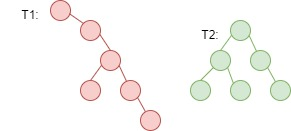
\includegraphics[width=0.5\textwidth ]{t1-1.jpg}
        %\caption{A boat.}
        %\label{fig:boat1}
    \end{figure}
    
    
        
    \item Demuestra que si un árbol $T_1$ puede ser \textsc{right-converted} a $T_2$, entonces $T_1$ puede ser \textsc{right-converted} usando $O(n^2)$ operaciones \textsc{right-rotate}.
    
    Sea $u$ un vértice en $T_1$ el cual tiene un vértice $u'$ el cual tiene un vértice $u'$ en $T_2$ de forma que despues de un número de operaciones \textsc{right-rotate} $u$ se encuentra en la posición de $u'$, esto le tomara en el peor de los casos $n$ (el número de vértices) por que ocupará el lugar de todos los vértices en $T_1$ antes de llegar a la posición de $u'$. En la figura siguiente podemos observar un ejemplo del movimiento.
    \begin{figure}[h!]
        \centering
        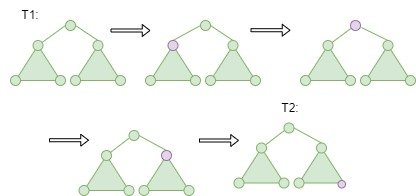
\includegraphics[width=0.6\textwidth]{t1-2.jpg}

        %\caption{A boat.}
        %\label{fig:boat1}
    \end{figure}
\end{itemize} 

Lo anterior es verdad para todos los $n$ vértices por ende si un árbol $T_1$ puede ser \textsc{right-converted} a $T_2$, entonces $T_1$ puede ser \textsc{right-converted} usando $O(n^2)$ operaciones \textsc{right-rotate}.

\bigskip
